\section{Abstract Theory}
Let $(X,\lVert\cdot\rVert_X)$ be a Banach space. Consider a functional
\[I:X\longrightarrow\mathbb{R}_\infty:=\mathbb{R}\cup\{+\infty\}.\]
The direct problem of calculus of variations is to find $u_0\in X$ with $I(u_0)=\inf_{u\in X}{I(u)}$. Such an element $u_0$ is called \textit{solution of the direct problem}. But how can we find minimizers? There is a standard recipe:
\begin{enumerate}
	\item First, consider an infimizing sequence $(u_n)_{n\in\mathbb{N}}\subset X$ such that $\lim_{n\to\infty}{I(u_n)}=\inf_{u\in X}{I(u)}$.
	\item Then ensure that $(u_n)_{n\in\mathbb{N}}$ is bounded.
	\item Then choose a subsequence $(u_{n_k})_{k\in\mathbb{N}}$ which converges in a suitable sense to some $u_*\in X$ and obtain $\lim_{k\to\infty}{I(u_{n_k})}=I(u_*)$.
\end{enumerate}
Then $u_0=u_*$ is a minimizer. In much applications, the functional $I$ satisfies a certain coercivity-property which ensures boundedness of any infimizing sequence.\\

\textbf{\underline{Definition 3.1.1}}\\
A functional $I:X\longrightarrow\mathbb{R}_\infty$ on a Banach space $X$ is called \textit{coercive} if $I(u)\to+\infty$ as $\lVert u\rVert_X\to+\infty$.\\[11pt]

\textbf{Proposition 3.1.2}\\
(Finite-dimensional case)\\
If $I:\mathbb{R}^m\longrightarrow\mathbb{R}_\infty$, $m\in\mathbb{N}$, is coercive and continuous, then the direct problem has a solution.\newpage

\textit{Proof:}\\
Let $(u_n)_{n\in\mathbb{N}}$ be an infimizing sequence. Coercivity implies that $(u_n)_{n\in\mathbb{N}}$ is bounded -- unless $I$ is infinity everywhere, but then the assertion it trivial. Then Bolzano-Weierstra{\ss} yields a convergent subsequence $u_{n_k}\to u_0$ as $k\to\infty$ for some $u_0\in\mathbb{R}^m$. Continuity of $I$ implies
\[I(u_0)=\lim_{k\to\infty}{I(u_{n_k})}=\inf_{u\in\mathbb{R}^m}{I(u)}.\]
\hfill$\blacksquare$\\[11pt]

In infinite dimensions:
\begin{itemize}
	\item[(a)] We cannot choose a convergent subsequence!
	\item[(b)] Continuity might not be suitable. For instance, consider
	\[I:\ell^2\longrightarrow\mathbb{R},\qquad x=(x_n)_{n\in\mathbb{N}}\longmapsto(1-\lVert x\rVert_{\ell^2}^2)^2+\sum_{k=1}^\infty{\frac{1}{k}x_k^2}.\]
	Then $I$ is a continuous and coercive functional, but in the exercises we have shown that $I$ admits no minimizer.\\
\end{itemize}

There are two ways out:
\begin{itemize}
	\item[(1)] Equip the functional $I$ with additional conditions that guarantee convergence in $\lVert\cdot\rVert_X$ and (norm-)continuity.
	\item[(2)] Find a suitable (weaker) notion of convergences in $X$ such that boundedness of a sequence implies convergence of a subsequence, and find conditions such that $I$ is continuous with respect to the new type of convergence.\\
\end{itemize}

First, we address variant (1).\\

\textbf{\underline{Definition 3.1.3}}\\
(Uniform convexity)\\
\begin{figure}[ht]
	\centering
	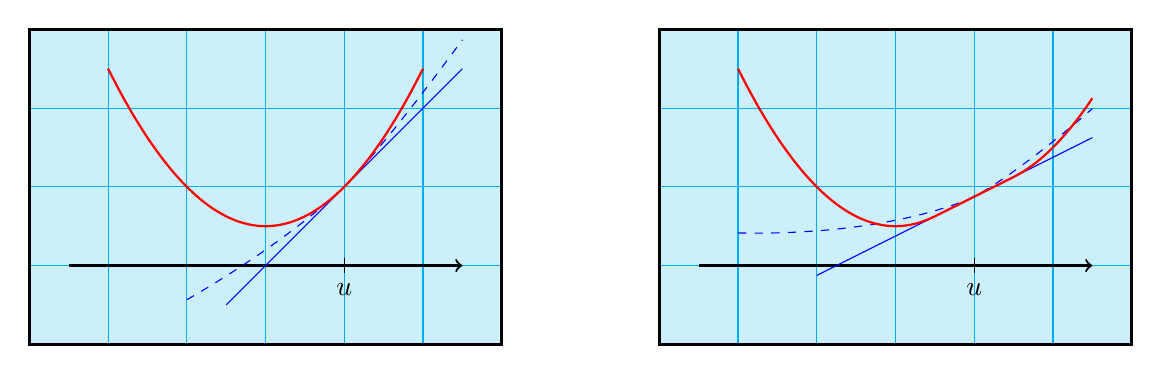
\begin{tikzpicture}
		% Hintergrund und Achsen
		\fill[cyan!20] (-7, -1) rectangle (-1, 3);
		\draw[cyan] (-7, -1) grid (-1, 3);
		\draw[thick, ->] (-6.5, 0) -- (-1.5, 0);
		\draw[thin] (-3, 0.1) -- (-3, -0.1) node[below] {$u$};
		\draw[very thick] (-7, -1) rectangle (-1, 3);

		% Funktionen
		\draw[blue] (-4.5, -0.5) -- (-1.5, 2.5);
		\draw[blue, dashed] plot[smooth, domain=-5:-1.5] (\x, {4+\x+0.2*abs(\x+3)^(3/2)});
		\draw[thick, red] plot[smooth, domain=-6:-2] (\x, {0.5+0.5*(\x+4)^2});

		% Hintergrund und Achsen
		\fill[cyan!20] (1, -1) rectangle (7, 3);
		\draw[cyan] (1, -1) grid (7, 3);
		\draw[thick, ->] (1.5, 0) -- (6.5, 0);
		\draw[thin] (5, 0.1) -- (5, -0.1) node[below] {$u$};
		\draw[very thick] (1, -1) rectangle (7, 3);

		% Funktionen
		\draw[blue] (3, -0.125) -- (6.5, 1.625);
		\draw[blue, dashed] plot[smooth, domain=2:6.5] (\x, {-1.625+\x*0.5+0.2*abs(\x-5)^(3/2)});
		\draw[thick, red] plot[smooth, domain=2:4.5] (\x, {0.5+0.5*(\x-4)^2});
		\draw[thick, red] (4.5, 0.625) -- (5.5, 1.125);
		\draw[thick, red] plot[smooth, domain=5.5:6.5] (\x, {1+0.5*(\x-5)^2});
	\end{tikzpicture}
	\caption{Illustration of uniform convexity (left) and non-uniform convexity (right).}
\end{figure}

We call $I:X\longrightarrow\mathbb{R}_\infty$ \textit{uniformly convex} if there is a function $g:[0,\infty)\longrightarrow\mathbb{R}$ with $g(0)=0$ which is strictly increasing such that for every $u\in X$ there exists a linear, continuous functional $L_u:X\longrightarrow\mathbb{R}$ satisfying
\[I(v)\geq I(u)+L_u(v-u)+g(\lVert u-v\rVert_X).\]

Very often, $g(t)=ct^p$ for some $p>1$, $c>0$ is appropriate.\\[11pt]

\textbf{\underline{Theorem 3.1.4}}\\
Let $I$ be uniformly convex and continuous with respect to $\lVert\cdot\rVert_X$. If $\inf_{u\in X}{I(u)}>-\infty$, then the direct problem has a solution. Moreover, if $I$ is not constantly $+\infty$, the solution is unique.\\

\textit{Proof:}\\
If $I$ is constantly $+\infty$ then the assertion is clear. So assume $I(u)<\infty$ for some $u\in X$ so that in particular $\alpha:=\inf_{u\in X}{I(u)}<\infty$. Let $(u_n)_{n\in\mathbb{N}}$ be an infimizing sequence, i.e. $\lim_{n\to\infty}{I(u_n)}=\alpha$. With the quantities $u=\frac{1}{2}(u_n+u_m)$ and $v=u_m$, the uniform convexity yields
\[I(u_m)\geq I\left(\frac{u_n+u_m}{2}\right)+L_{\frac{1}{2}(u_n+u_m)}\left(\frac{1}{2}(u_m-u_n)\right)+g\left(\frac{1}{2}\lVert u_n-u_m\rVert_X\right),\]
and exchanging $n$ and $m$,
\[I(u_n)\geq I\left(\frac{u_n+u_m}{2}\right)+L_{\frac{1}{2}(u_n+u_m)}\left(\frac{1}{2}(u_n-u_m)\right)+g\left(\frac{1}{2}\lVert u_m-u_n\rVert_X\right).\]
Summing up, we have
\[I(u_m)+I(u_n)\geq 2I\left(\frac{u_n+u_m}{2}\right)+2g\left(\frac{1}{2}\lVert u_n-u_m\rVert_X\right)\geq 2\alpha+2g\left(\frac{1}{2}\lVert u_n-u_m\rVert_X\right).\]
The left-hand side converges to $2\alpha$ as $m,n\to\infty$. Hence, $g\left(\frac{1}{2}\lVert u_n-u_m\rVert_X\right)\to0$ as $m,n\to\infty$. Strict monotonicity implies $\lVert u_n-u_m\rVert_X\to0$ as $m,n\to\infty$ so that $(u_n)_{n\in\mathbb{N}}$ is a Cauchy sequence. Thus, $(u_n)_{n\in\mathbb{N}}$ converges to some limit $u_*\in X$. Continuity implies $I(u_*)=\lim_{n\to\infty}{I(u_n)}=\inf_{u\in X}{I(u)}$. Hence $u_*$ is a minimizer.\\

If $v_*$ would be another minimizer, then $I(u_*)=I(v_*)$ and
\begin{align*}
	I(u_*)&\geq I\left(\frac{u_*+v_*}{2}\right)+L_{\frac{1}{2}(u_*+v_*)}\left(\frac{1}{2}(u_*-v_*)\right)+g\left(\frac{1}{2}\lVert u_*-v_*\rVert_X\right),\\
	I(v_*)&\geq I\left(\frac{u_*+v_*}{2}\right)+L_{\frac{1}{2}(u_*+v_*)}\left(\frac{1}{2}(v_*-u_*)\right)+g\left(\frac{1}{2}\lVert u_*-v_*\rVert_X\right).
\end{align*}
Therefore
\[2I(u_*)=I(u_*)+I(v_*)\geq 2I\left(\frac{u_*+v_*}{2}\right)+2g\left(\frac{1}{2}\lVert u_*-v_*\rVert_X\right)\geq 2I(u_*)+2g\left(\frac{1}{2}\lVert u_*-v_*\rVert_X\right),\]
hence $g\left(\frac{1}{2}\lVert u_*-v_*\rVert_X\right)\leq0$, i.e. $u_*=v_*$.\hfill$\blacksquare$\\[11pt]

In many applications, the assumption of uniform convexity is too restrictive. It is rather exceptional. Our next goal is to follow the second variant, i.e. to develop a weaker notion of convergence. For that, we start with a short revision from functional analysis to fix the notation.\newpage

\textbf{\underline{Definition 3.1.5}}\\
Let $X$ be a Banach space.
\begin{itemize}
	\item[(i)] The vector space $X':=\mathcal{L}(X,\mathbb{R})=\{\varphi:X\longrightarrow\mathbb{R}\text{ linear, continuous}\}$ is called the \textit{dual space of $X$}. It is equipped with the norm
	\[\lVert\varphi\rVert_{X'}:=\sup_{\lVert x\rVert_X\leq1}{\lvert\varphi(x)\rvert}\quad\left(=\sup_{\lVert x\rVert_X=1}{\lvert\varphi(x)\rvert}\quad\text{if }\dim(X)>0\right).\]
	\item[(ii)] A sequence $(u_n)_{n\in\mathbb{N}}\subset X$ is said to \textit{converge weakly to $u$ in $X$} for some $u\in X$ if for all $\varphi\in X'$ we have $\varphi(u_n)\to\varphi(u)$ as $n\to\infty$. The notation is $u_n\rightharpoonup u$. (In contrast to $u_n\to u$ for convergence with respect to norm $\lVert\cdot\rVert_X$.)
	\item[(iii)] The dual space of $X'$ is denoted by $X''=(X')'$ and is called the \textit{bidual space of $X$}.\\[11pt]
\end{itemize}

\textbf{\underline{Theorem 3.1.6}}\\
(Riesz representation theorem)\\
Let $X$ be a Hilbert space. Then for all $\varphi\in X'$ there exists a unique $v_\varphi\in X$ such that for all $u\in X$ it holds $\varphi(u)=\langle v_\varphi,u\rangle$ with $\langle\cdot,\cdot\rangle$ being the scalar product in $X$. Moreover, the map
\[X'\overset{\sim}{\longrightarrow}X,\qquad\varphi\longmapsto v_\varphi\]
is an isometric isomorphism.\\

In particular, a sequence $(u_n)_{n\in\mathbb{N}}\subset X$ converges weakly to $u\in X$ in $X$ if and only if $\langle v,u_n\rangle\to\langle v,u\rangle$ as $n\to\infty$, for all $v\in X$.\\

\textit{Proof:}\\
This is a standard result from functional analysis.\hfill$\blacksquare$\\[11pt]

\hypertarget{remark_3_1_7}{\textbf{Remark 3.1.7}}\\
The following facts are also shown in functional analysis course.
\begin{itemize}
	\item[(a)] The weak limit of a weakly convergent sequence is unique. That's a consequence from Hahn-Banach.
	\item[(b)] Strong convergence, i.e. norm convergence $u_n\to u$, implies weak convergence $u_n\rightharpoonup u$.
	\item[(c)] Weakly convergent sequences are bounded.
	\item[(d)] If $(u_n)_{n\in\mathbb{N}}\subset X$ converges weakly to some $u\in X$ in $X$ then
	\[\lVert u\rVert_X\leq\liminf_{n\to\infty}{\lVert u_n\rVert_X}.\]
	\item[(e)] A Banach space $X$ is naturally embedded into its bidual $X''$ via
	\[J:X\longhookrightarrow X'',\qquad J(u)=[X'\longrightarrow\mathbb{R},\quad\varphi\longmapsto J(u)(\varphi):=\varphi(u)].\]
	This map is isometric and hence injective in general, but not surjective.\\[11pt]
\end{itemize}

\textbf{\underline{Definition 3.1.8}}\\
A Banach space $X$ is called \textit{reflexive} if $J$ is surjective, i.e. if the map from \hyperlink{remark_3_1_7}{Remark 3.1.7 (e)} is an isometric isomorphism.\\[11pt]

\hypertarget{theorem_3_1_9}{\textbf{\underline{Theorem 3.1.9}}}\\
(Eberlin-\v{S}mulian)\\
A Banach space $X$ is reflexive if and only if every bounded sequence $(u_n)_{n\in\mathbb{N}}\subset X$ contains a weakly convergent subsequence.\\

\textit{Remark: The statement from Eberlin-\v{S}mulian tells us that weak compactness is the same as sequential weak compactness.}\\

\textit{Proof:}\\
This is also done in linear functional analysis.\hfill$\blacksquare$\\[11pt]

\textbf{\underline{Definition 3.1.10}}\\
A (nonlinear) functional $I:X\longrightarrow\mathbb{R}_\infty$ is called \textit{weakly (sequentially) continuous} if for all $(u_n)_{n\in\mathbb{N}}\subset X$, $u\in X$ with $u_n\rightharpoonup u$ (as $n\to\infty$) it follows $\lim_{n\to\infty}{I(u_n)}=I(u)$.\\[11pt]

\textbf{Remark 3.1.11}
\begin{itemize}
	\item[(a)] If $I$ is weakly sequentially continuous then it is also strongly (sequentially) continuous. The latter just means continuity with respect to $\lVert\cdot\rVert_X$.
	\item[(b)] There are ``not many'' weakly sequentially continuous functions.
	\item[(c)] Normally, continuity is defined via open sets, i.e. preimages of open sets have to be open. But we work with sequences in the definition, and that's why we should write ``sequentially'' all the time. However, we will drop this from now on because we will always work with sequences.\\[11pt]
\end{itemize}

\hypertarget{examples_3_1_12}{\textbf{Examples 3.1.12}}
\begin{itemize}
	\item[(a)] Consider $X=\ell^2$ and $I(u):=\lVert u\rVert_{\ell^2}^2=\sum_{k=1}^\infty{u_k^2}$. This is a reasonable function and we already know that this has a unique minimizer, namely $I(0)=0$. However, $I$ is not weakly continuous. Consider $u^{(n)}=(0,\dotsc,0,1,0,\dotsc)$ where the 1 appears only at the $n$-th position. Then $u^{(n)}\rightharpoonup0$ as $n\to\infty$ in $\ell^2$, but $I(u^{(n)})=1\not\to0$ for $n\to\infty$.
	\item[(b)] Consider $f\in C^0(\overline{\Omega}\times\mathbb{R}^m)$ that satisfies the growth property: There exists $C>0$, $p\in[1,\infty)$ and $h\in L^1(\Omega)$ such that
	\[\lvert f(x,u)\rvert\leq C(h(x)+\lvert u\rvert^p)\]
	for all $(x,u)\in\Omega\times\mathbb{R}^m$. Define the functional
	\[I:L^p(\Omega;\mathbb{R}^m)\longrightarrow\mathbb{R},\qquad I(u):=\int_\Omega{f(x,u(x))\mathrm{d}x}.\]
	In this setting, one can show that $I$ is always strongly continuous (i.e. this will be shown in the exercises). But $I$ is weakly continuous if and only if $f(x,\cdot)$ is affine, i.e., there exist $a\in C^0(\overline{\Omega})$ and $b\in C^0(\overline{\Omega};\mathbb{R}^m)$ such that $f(x,u)=a(x)+b(x)\cdot u$.\newpage
\end{itemize}

So we see that the notion of weak continuity is not a good choice. We need to relax it.\\[11pt]

\textbf{\underline{Definition 3.1.13}}\\
A functional $I:X\longrightarrow\mathbb{R}_\infty$ is called \textit{weakly (sequentially) lower semicontinuous} if for all $(u_n)_{n\in\mathbb{N}}\subset X$, $u\in X$ with $u_n\rightharpoonup u$ in $X$ as $n\to\infty$, it follows
\[I(u)\leq\liminf_{n\to\infty}{I(u_n)}.\]

\begin{figure}[ht]
	\centering
	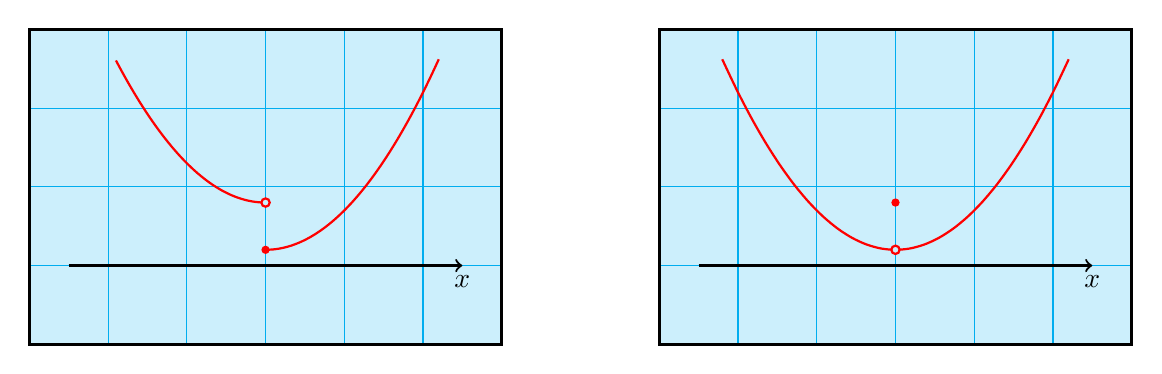
\begin{tikzpicture}
		% Hintergrund und Achsen
		\fill[cyan!20] (-7, -1) rectangle (-1, 3);
		\draw[cyan] (-7, -1) grid (-1, 3);
		\draw[thick, ->] (-6.5, 0) -- (-1.5, 0) node[below] {$x$};
		\draw[very thick] (-7, -1) rectangle (-1, 3);

		% Funktionen
		\draw[thick, red] plot[smooth, domain=-5.9:-4] (\x, {0.8+(\x+4)^2/2});
		\draw[thick, red] plot[smooth, domain=-4:-1.8] (\x, {0.2+(\x+4)^2/2});
		\draw[thick, red, fill=cyan!20] (-4, 0.8) circle (1.5pt);
		\fill[red] (-4, 0.2) circle (1.5pt);

		% Hintergrund und Achsen
		\fill[cyan!20] (1, -1) rectangle (7, 3);
		\draw[cyan] (1, -1) grid (7, 3);
		\draw[thick, ->] (1.5, 0) -- (6.5, 0) node[below] {$x$};
		\draw[very thick] (1, -1) rectangle (7, 3);

		% Funktionen
		\draw[thick, red] plot[smooth, domain=1.8:6.2] (\x, {0.2+(\x-4)^2/2});
		\draw[thick, red, fill=cyan!20] (4, 0.2) circle (1.5pt);
		\fill[red] (4, 0.8) circle (1.5pt);
	\end{tikzpicture}
	\caption{Example of a function which is lower semicontinuous (left) and not (right).}
\end{figure}

In general, the norm in a Banach space is not weakly continuous by \hyperlink{examples_3_1_12}{Examples 3.1.12 (a)}. But it is weakly lower semicontinuous by \hyperlink{remark_3_1_7}{Remark 3.1.7 (d)}.\\

\hypertarget{theorem_3_1_14}{\textbf{\underline{Theorem 3.1.14}}}\\
(Abstract existence theorem)\\
Let $X$ be a reflexive Banach space. Let $I:X\longrightarrow\mathbb{R}_\infty$ be coercive and weakly lower semicontinuous. Then the direct problem has a solution.\\

\textit{Proof:}\\
Let $\alpha:=\inf_{u\in X}{I(u)}$. If $\alpha=\infty$ then $I(u)=+\infty$ for all $u\in X$, so every $u\in X$ is a minimizer. Now let us assume $\alpha<\infty$. By definition, there exists an infimizing sequence $(u_n)_{n\in\mathbb{N}}\subset X$, i.e. $\lim_{n\to\infty}{I(u_n)}=\alpha$. Since $\alpha<\infty$, we have $I(u_n)\leq C<\infty$ for some $C\in\mathbb{R}$ and large $n$. Coercivity implies that $(u_n)_{n\in\mathbb{N}}$ is bounded in $X$. Theorem from Eberlein-\v{S}mulian, i.e. \hyperlink{theorem_3_1_9}{Theorem 3.1.9}, yields a weakly convergent subsequence $(u_{n_k})_{k\in\mathbb{N}}\subset(u_n)_{n\in\mathbb{N}}$. Let $u_*\in X$ be the weak limit. Since $I$ is weakly lower semicontinuous, we obtain
\[\inf_{u\in X}{I(u)}\leq I(u_*)\leq\liminf_{k\to\infty}{I(u_{n_k})}=\alpha=\inf_{u\in X}{I(u)}.\]
\hfill$\blacksquare$\\[11pt]

We see that lower weak semicontinuity fits perfectly into our setting. This motivates to study this continuity-type a bit more and to find equivalent notions.\\[11pt]

\hypertarget{theorem_3_1_15}{\textbf{\underline{Theorem 3.1.15}}}\\
Let $X$ be a Banach space, $I:X\longrightarrow\mathbb{R}_\infty$. The following statements are equivalent.
\begin{itemize}
	\item[(i)] $I$ is $\left\{\begin{array}{l}
		\text{(strongly) lower semicontinuous}\\
		\text{weakly lower semicontinuous}
	\end{array}\right\}$.
	Strong lower semicontinuity means that for all $(u_n)_{n\in\mathbb{N}}\subset X$, $u\in X$ with $u_n\to u$ in $X$ we have $I(u)\leq\liminf_{n\to\infty}{I(u_n)}$.
	\item[(ii)] The epigraph of $I$ is $\left\{\begin{array}{l}
		\text{strongly sequentially closed}\\
		\text{weakly sequentially closed}
	\end{array}\right\}$.

	The epigraph is defined as $\epi{I}:=\{(u,\alpha)\in X\times\mathbb{R}\mid I(u)\leq\alpha\}$.
	\item[(iii)] The sublevel sets of $I$ are $\left\{\begin{array}{l}
		\text{strongly sequentially closed}\\
		\text{weakly sequentially closed}
	\end{array}\right\}$.

	The sublevel sets are all the sets of the form $S_\alpha(I):=\{u\in X\mid I(u)\leq\alpha\}$ with $\alpha\in\mathbb{R}$.\\
\end{itemize}

\textit{Proof:}\\
In the following, ``$\rightsquigarrow$'' denotes either strong or weak convergence because the arguments are always the same.
\begin{itemize}
	\item[(i)] $\Rightarrow$ (ii): Take a sequence $(u_n,\alpha_n)_{n\in\mathbb{N}}\subset\epi{I}$ such that $u_n\rightsquigarrow u$ in $X$ and $\alpha_n\to\alpha$ in $\mathbb{R}$ for some $u\in X$, $\alpha\in\mathbb{R}$. Then
	\[\alpha=\lim_{n\to\infty}{\alpha_n}\geq\liminf_{n\to\infty}{I(u_n)}\geq I(u),\]
	hence $(u,\alpha)\in\epi{I}$.
	\item[(ii)] $\Rightarrow$ (iii): Let $\alpha\in\mathbb{R}$ and $(u_n)_{n\in\mathbb{N}}\subset S_\alpha(I)$ such that $u_n\rightsquigarrow u$ in $X$ for some $u\in X$. Then $(u_n,\alpha)\rightsquigarrow(u,\alpha)$ in $X\times\mathbb{R}$. Since $(u_n,\alpha)\in\epi{I}$ for all $n\in\mathbb{N}$ and $\epi{I}$ is closed with respect to ``$\rightsquigarrow$'', we have $(u,\alpha)\in\epi{I}$, so $I(u)\leq\alpha$, so $u\in S_\alpha(I)$.
	\item[(iii)] $\Rightarrow$ (i): Let $(u_n)_{n\in\mathbb{N}}\subset X$, $u\in X$ such that $u_n\rightsquigarrow u$ in $X$ for $n\to\infty$, and write $c:=\liminf_{n\to\infty}{I(u_n)}$. If $c=\infty$ then $I(u)\leq\infty$ trivially and we have nothing to do. If $c<\infty$, then consider a subsequence $(u_{n_k})_{k\in\mathbb{N}}\subset(u_n)_{n\in\mathbb{N}}$ with $c=\lim_{k\to\infty}{I(u_{n_k})}$.\\

	For all $\alpha>c$, there exists $K_\alpha$ such that $I(u_{n_k})\leq\alpha$ for all $k\geq K_\alpha$. This means $u_{n_k}\in S_\alpha(I)$ for all $k\geq K_\alpha$, and since $S_\alpha(I)$ is closed with respect to ``$\rightsquigarrow$'', we obtain $u\in S_\alpha(I)$, i.e. $I(u)\leq\alpha$ for all $\alpha>c$. This means nothing else but
	\[I(u)\leq c=\lim_{k\to\infty}{I(u_{n_k})}=\liminf_{n\to\infty}{I(u_n)}.\]
	\hfill$\blacksquare$\\[11pt]
\end{itemize}

We want to learn more about weakly lower semicontinuous functions. The question about this property for a functional $I$ can be turned over by \hyperlink{theorem_3_1_15}{Theorem 3.1.15} to the question, when the sublevel sets are weakly sequentially closed. It turns out that convex functionals play an important role.